\chapter{Results}
\textit{\ifdraft{In this section you discuss any issues that came up while developing
the system.  If you found something particularly interesting,
difficult, or an important learning experience, put it here.  This is
also a good place to put additional figures and data.}}

\section{Using a robot to create image dataset}\label{resrobotcontrol}

\subsection*{Tests}
Robot manipulator performance was measured by making four tests and taking time, iterations and interventions. The performance can been seen in \textit{Table \ref{tab:testonrobot}}.

\begin{table}[h]
\resizebox{\textwidth}{!}{%
\begin{tabular}{clccccccc}
\hline
\textit{Test\#} &
  \textit{Item} &
  \textit{\begin{tabular}[c]{@{}c@{}}Start pos\\ {[}x, y, z{]}\end{tabular}} &
  \textit{Iterations} &
  \textit{\begin{tabular}[c]{@{}c@{}}Operator\\ intervention\end{tabular}} &
  \textit{\begin{tabular}[c]{@{}c@{}}Time \\ {[}sec{]}\end{tabular}} &
  \textit{\begin{tabular}[c]{@{}c@{}}Did it \\ finish?\end{tabular}} &
  \textit{\begin{tabular}[c]{@{}c@{}}Movement \\ time {[}sec{]}\end{tabular}} &
  \textit{\begin{tabular}[c]{@{}c@{}}Intervention\\ vs.  Iterations\end{tabular}} \\ \hline
\multicolumn{1}{c|}{1} &
  \begin{tabular}[c]{@{}l@{}}Nivea \\ Cleansing Milk\end{tabular} &
  \begin{tabular}[c]{@{}c@{}}{[}0.336, \\ 0.045, \\ 0.097{]}\end{tabular} &
  100 &
  2 &
  1277.2 &
  Yes &
  12.77 &
  2\% \\
\multicolumn{1}{c|}{2} &
  \begin{tabular}[c]{@{}l@{}}Alberto \\ Balsam coconut\end{tabular} &
  \begin{tabular}[c]{@{}c@{}}{[}0.343, \\ 0.043, \\ 0.107{]}\end{tabular} &
  100 &
  0 &
  1254.2 &
  Yes &
  12.54 &
  0\% \\
\multicolumn{1}{c|}{3} &
  \begin{tabular}[c]{@{}l@{}}Nivea \\ Cleansing Milk\end{tabular} &
  \begin{tabular}[c]{@{}c@{}}{[}0.340 , \\ 0.044, \\ 0.098{]}\end{tabular} &
  300 &
  6 &
  3799.1 &
  Yes &
  12.66 &
  2\%  \\
\multicolumn{1}{c|}{4} &
  \begin{tabular}[c]{@{}l@{}}Alberto \\ Balsam coconut\end{tabular} &
  \begin{tabular}[c]{@{}c@{}}{[}0.333 , \\ -0.040, \\ 0.118{]}\end{tabular} &
  300 &
  1 &
   3774.4&
  Yes &
   12.58 &
  0.33\% \\ \hline
\multicolumn{7}{r}{\textbf{Average:}} &
  12.64 &
  1.08\% \\ \hline
\end{tabular}%
}
\caption{Test made on the robot and code performance}
\label{tab:testonrobot}
\end{table}
\clearpage
%%%%%%%%%%%%%%%%%%%%%%%%%%%%%%%%%%%%%%%%%%%%%%%%%%%%%%%%%%%%%%%%%%%%%
\section{Automatic labelling}\label{rescamera}
The automatic labelling is not simple, since you need to look at few things such as lighting conditions, light reflection from objects, shades and more. So two methods were tested that were described in the methods chapter. 
\subsection{Before vs. after}
The results from the Before and After method was fine, but in some cases when the bottles area intersect each other it can't find the right bounding box. 
\begin{figure}[ht]
    \centering
    % include first image
    \subfloat[Before]{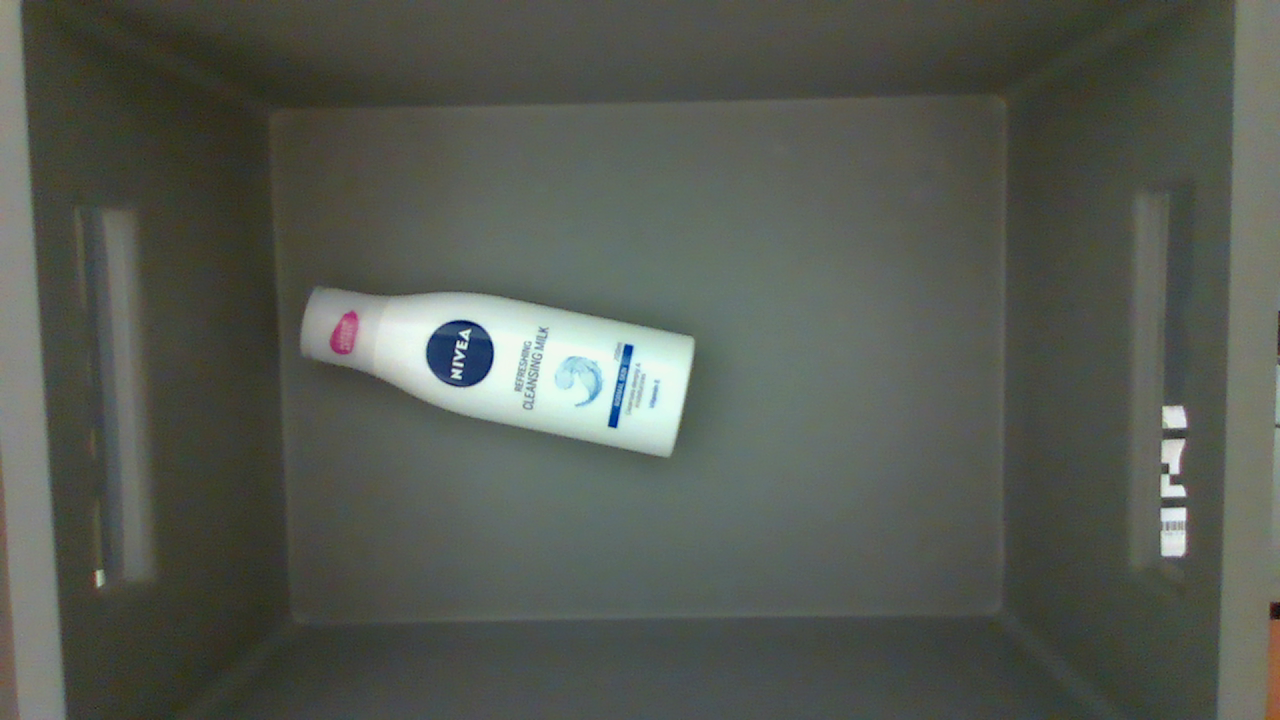
\includegraphics[width=0.495\textwidth]{graphics/9before.png}}
    \hfill
    \subfloat[After]{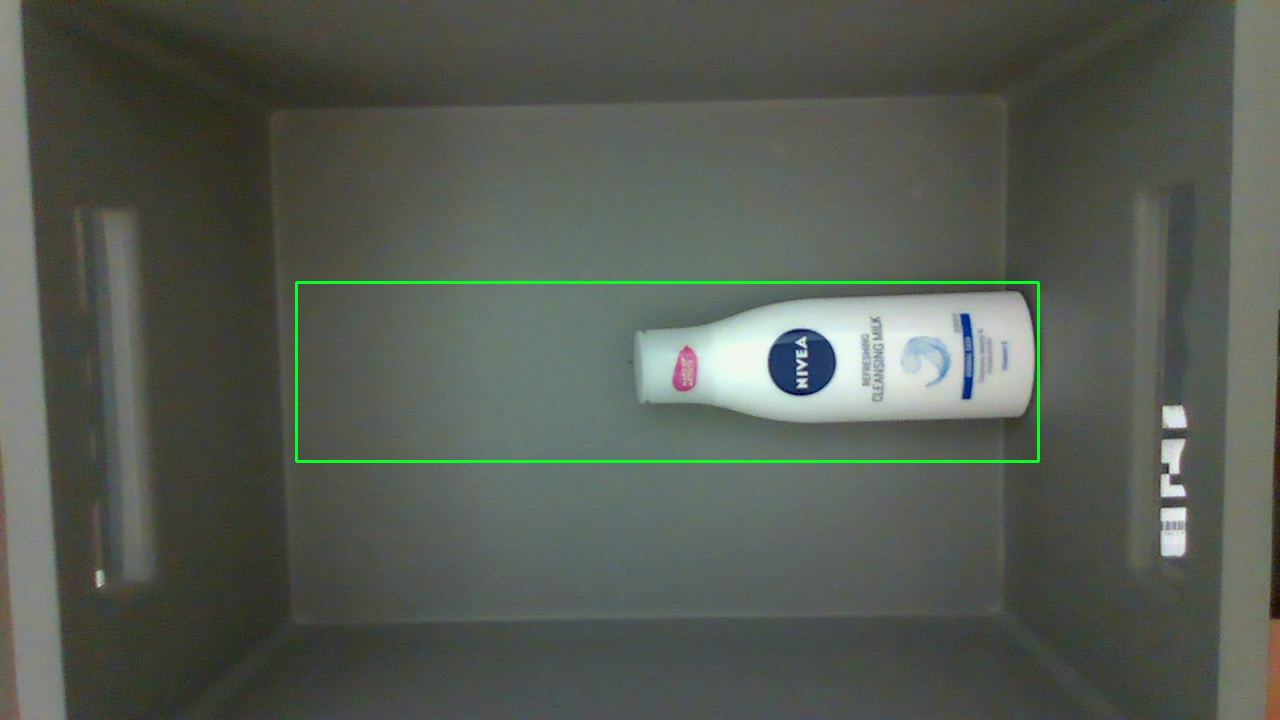
\includegraphics[width=0.495\textwidth]{graphics/9after.png}}
    \hfill
    \subfloat[Filled]{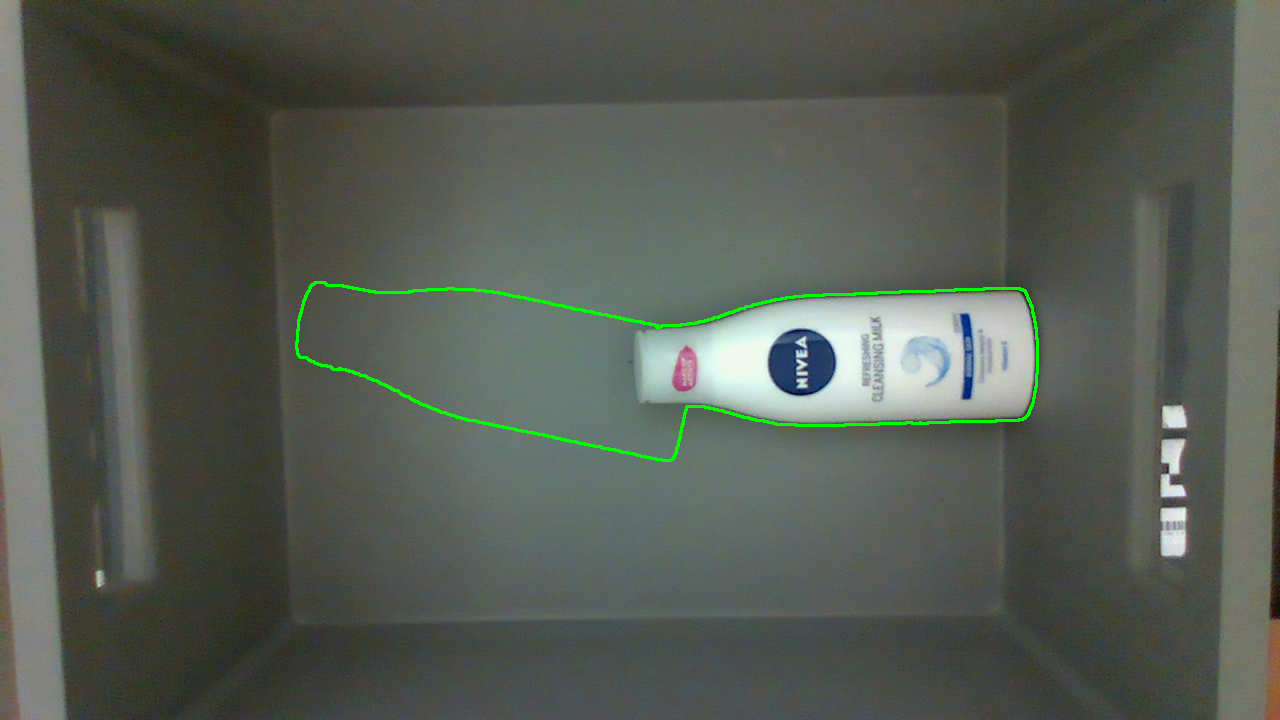
\includegraphics[width=0.495\textwidth]{graphics/9filled.png}}
    \hfill
    \subfloat[Masked]{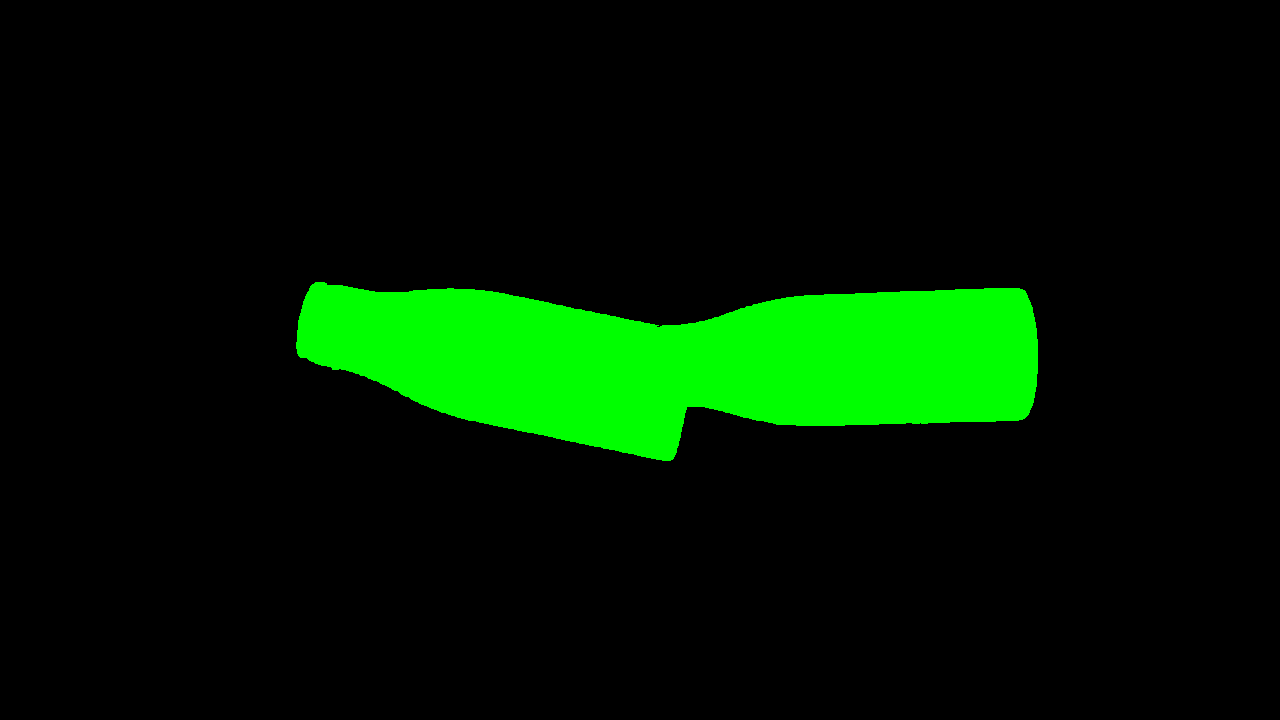
\includegraphics[width=0.495\textwidth]{graphics/9masked.png}}
    \caption{Image Difference with OpenCV and Python}
    \label{figure: imagework}
\end{figure}

As can been seen in the \textit{Figure \ref{figure: imagework}} this would not work so another method would be needed to find the right bounding box automatically. 

\subsection{Empty bin vs. Object in the bin}
The second method showed an increase in performance and almost perfect results, since it needed to go through two functions of object finding. So it would work for dark items, light items or strange shaped items.

As can been seen in the \textit{Figure \ref{figure: labelling}} this method works to create a automatic labelled data.

\begin{figure}[h]
    \centering
    % include first image
    \subfloat[Alberto Balsam]{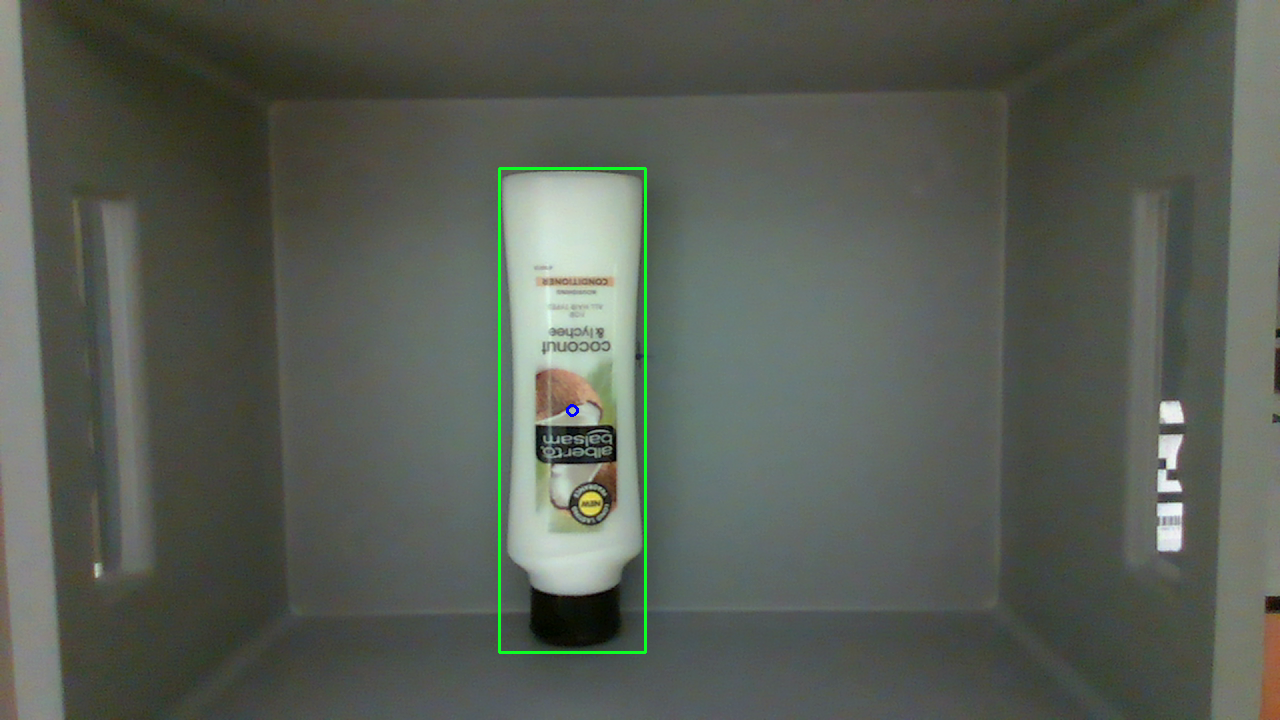
\includegraphics[width=0.495\textwidth]{graphics/results/albertobalsam100_51.png}}
    \hfill
    \subfloat[Nivea Cleansing Milk]{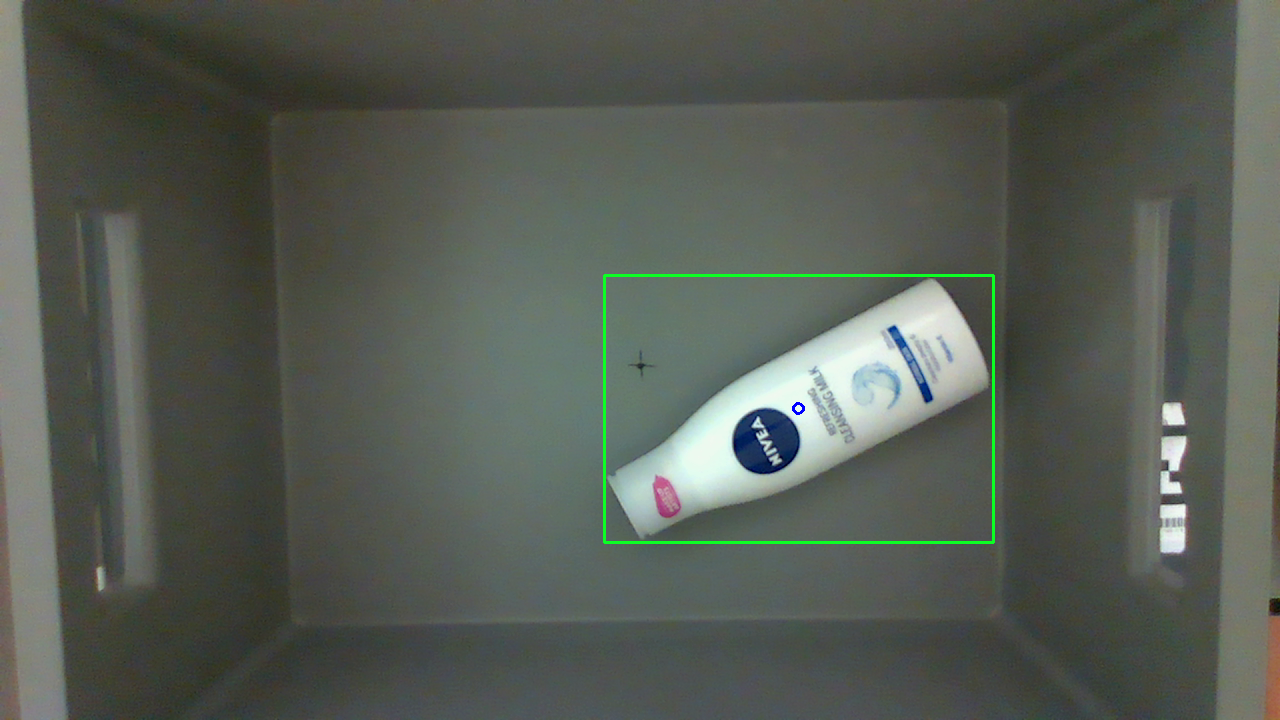
\includegraphics[width=0.495\textwidth]{graphics/results/niveacleansingmilk100_8.png}}
    \hfill
    \subfloat[Nivea Elastic]{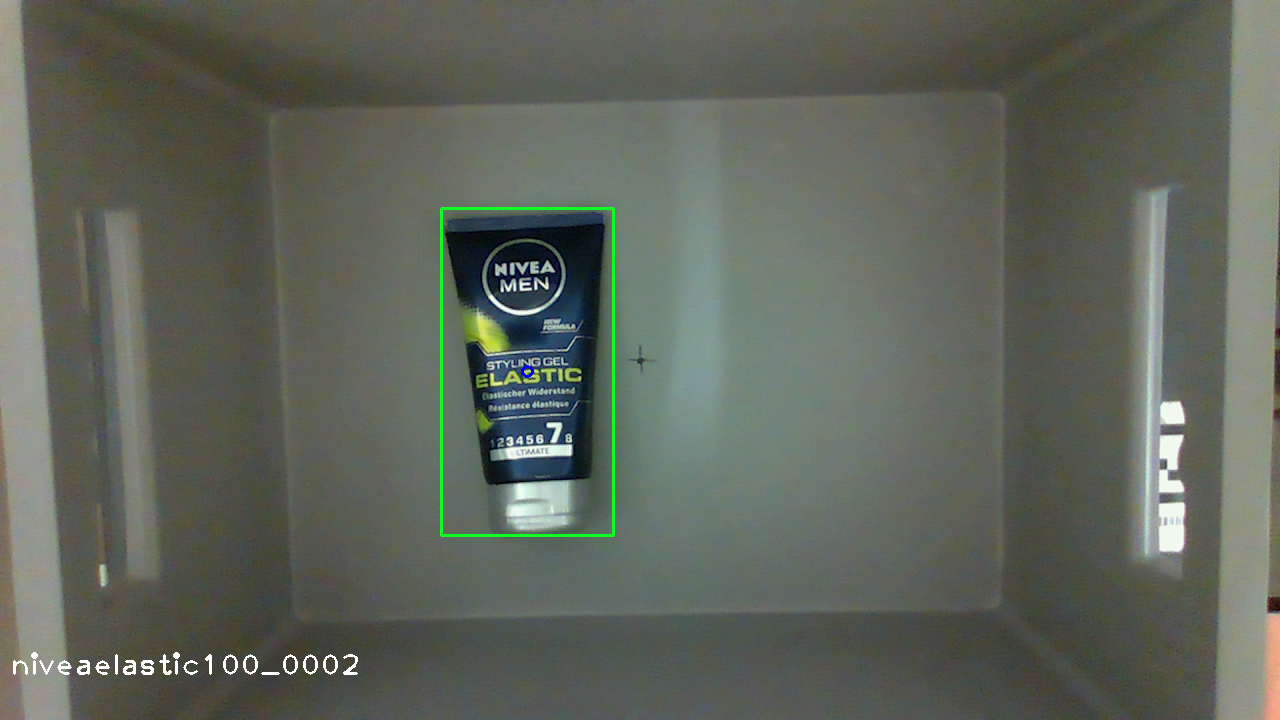
\includegraphics[width=0.495\textwidth]{graphics/results/niveaelastic100_0002box.png}}
    \hfill
    \subfloat[Nivea texture]{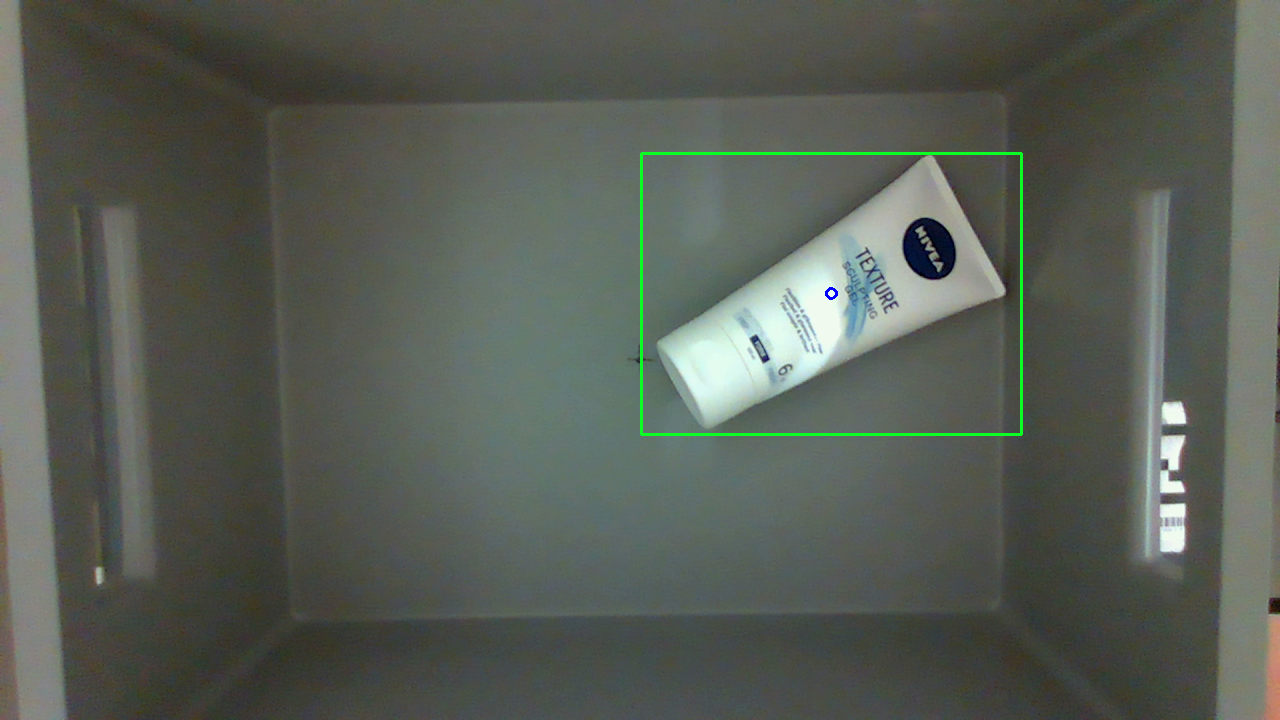
\includegraphics[width=0.495\textwidth]{graphics/results/niveatexture70_27.png}}
    \caption{The results from the difference.py, which shows the bounding box of four products}
    \label{figure: labelling}
\end{figure}


Since this method worked to created automatic labelled data, an test was made on the code how long would it take to label one image. Results from that test can been seen in \textit{Table \ref{tab:timediff}} and there it can be seen that it takes on average 0.85 second to label one image. 
\vspace{1cm}

\begin{table}[h]
\resizebox{\textwidth}{!}{%
\begin{tabular}{clccc}
\multicolumn{1}{l|}{\textit{Test \#}} &
  \textit{Item} &
  \multicolumn{1}{l}{\textit{Images}} &
  \multicolumn{1}{l}{\textit{Time {[}s{]}}} &
  \multicolumn{1}{l}{\textit{Time per image {[}s{]}}} \\ \hline
\multicolumn{1}{c|}{1} & \begin{tabular}[c]{@{}l@{}}Nivea\\ cleansing milk\end{tabular}    & 300 & 255.99 & 0.85 \\
\multicolumn{1}{c|}{2} & \begin{tabular}[c]{@{}l@{}}Nivea\\ cleansing milk\end{tabular}    & 102 & 92.68  & 0.91 \\
\multicolumn{1}{c|}{3} & \begin{tabular}[c]{@{}l@{}}Nivea \\ elastic\end{tabular}          & 72  & 56.31  & 0.78 \\
\multicolumn{1}{c|}{4} & \begin{tabular}[c]{@{}l@{}}Alberto \\ Balsam cocunut\end{tabular} & 102 & 88.30  & 0.87 \\ \hline
\multicolumn{4}{r}{Average:}                                                                              & 0.85
\end{tabular}%
}
\caption{Measured time when using the difference.py}
\label{tab:timediff}
\end{table}

\clearpage
%%%%%%%%%%%%%%%%%%%%%%%%%%%%%%%%%%%%%%%%%%%%%%%%%%%%%%%%%%%%%%%%%%%%%
\section{Creating a new model for object detection}\label{reslabelled}
\begin{figure}[h]
    \centering
    % include first image
    \subfloat[Using YOLOv4]{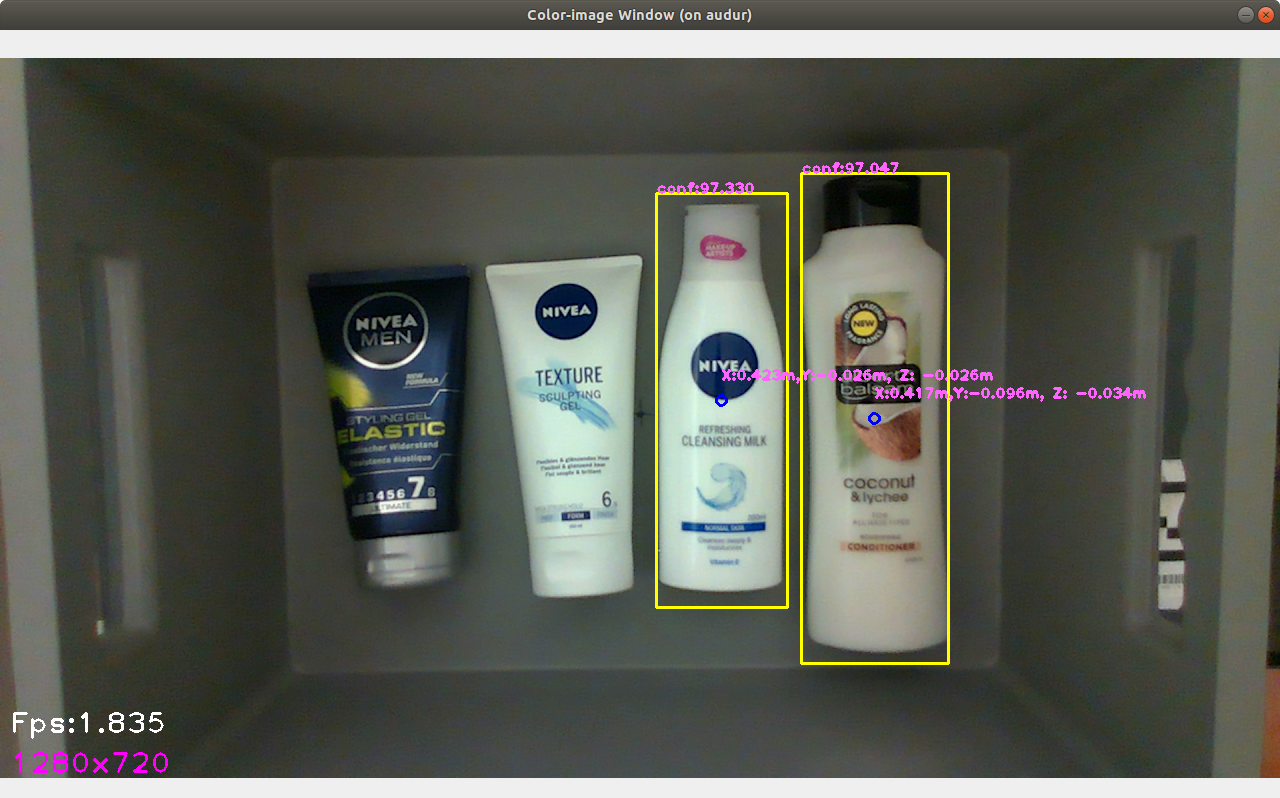
\includegraphics[width=0.33\textwidth]{graphics/results/beforetraining.png}}
    \hfill
    \subfloat[Using YOLOv4]{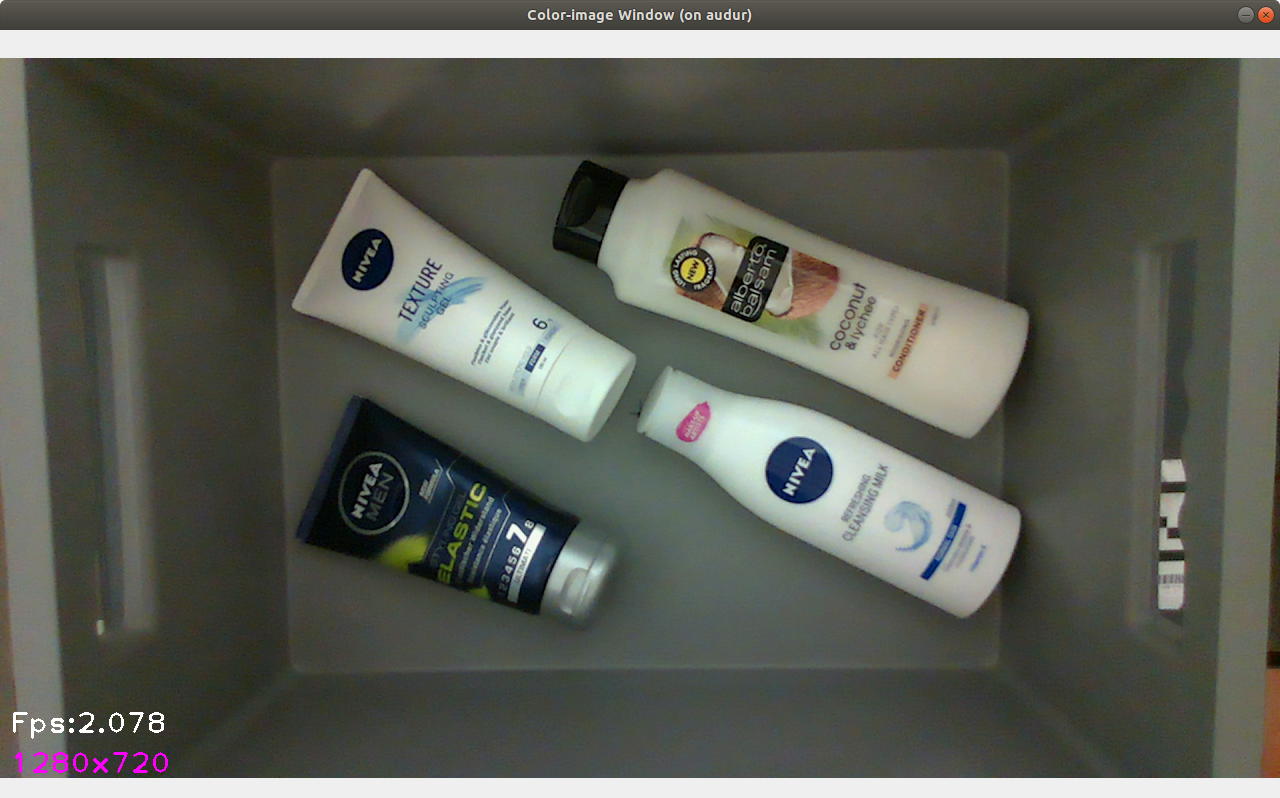
\includegraphics[width=0.33\textwidth]{graphics/results/beforetraining1.png}}
    \hfill
    \subfloat[Using YOLOv4]{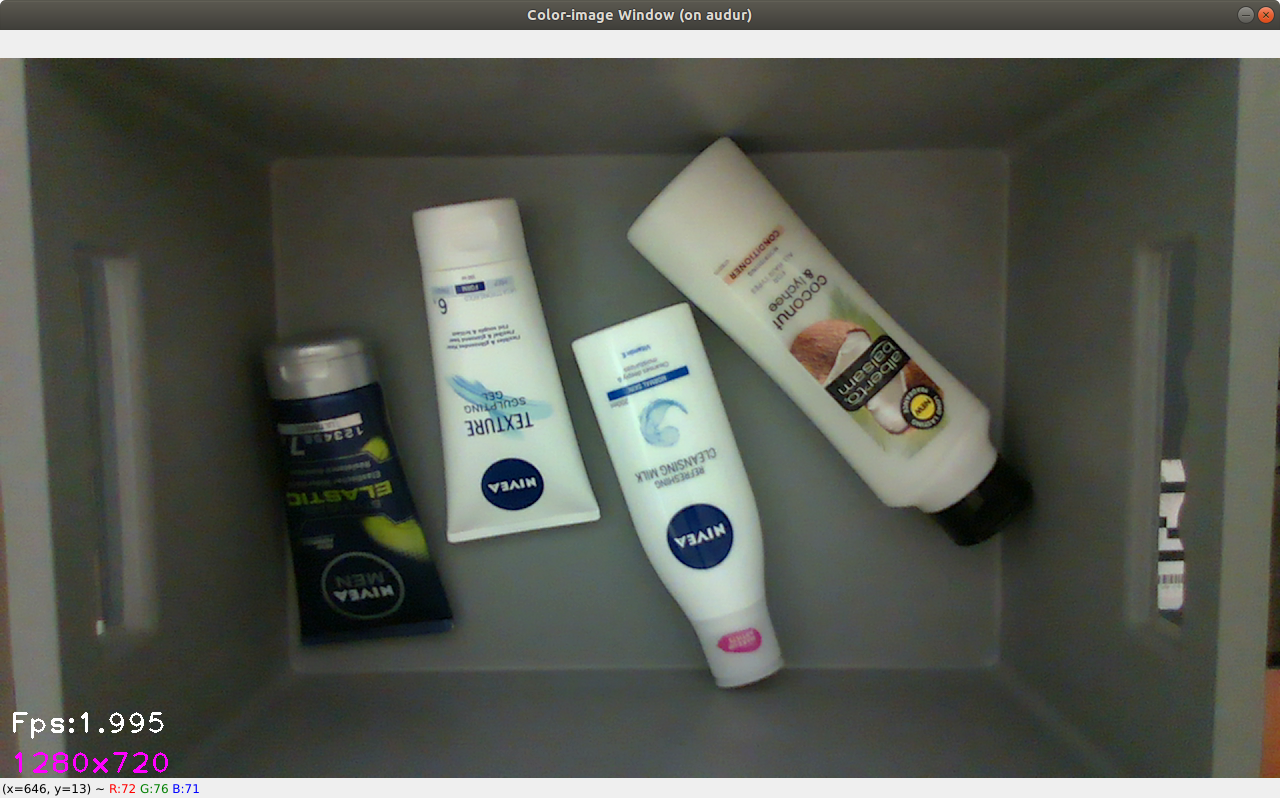
\includegraphics[width=0.33\textwidth]{graphics/results/beforetraining2.png}}
    \hfill
    \subfloat[Using trained YOLOv4]{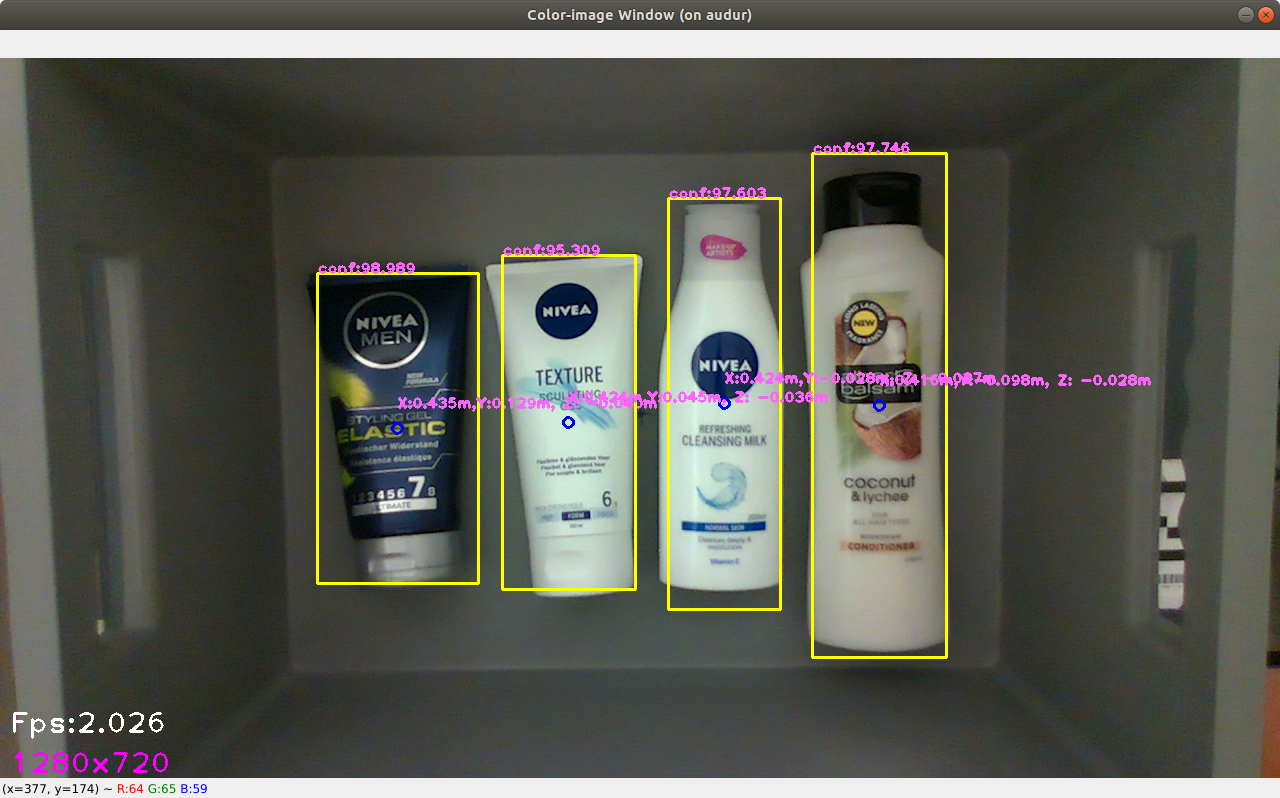
\includegraphics[width=0.33\textwidth]{graphics/results/aftertraining.png}}
    \hfill
    \subfloat[Using trained YOLOv4]{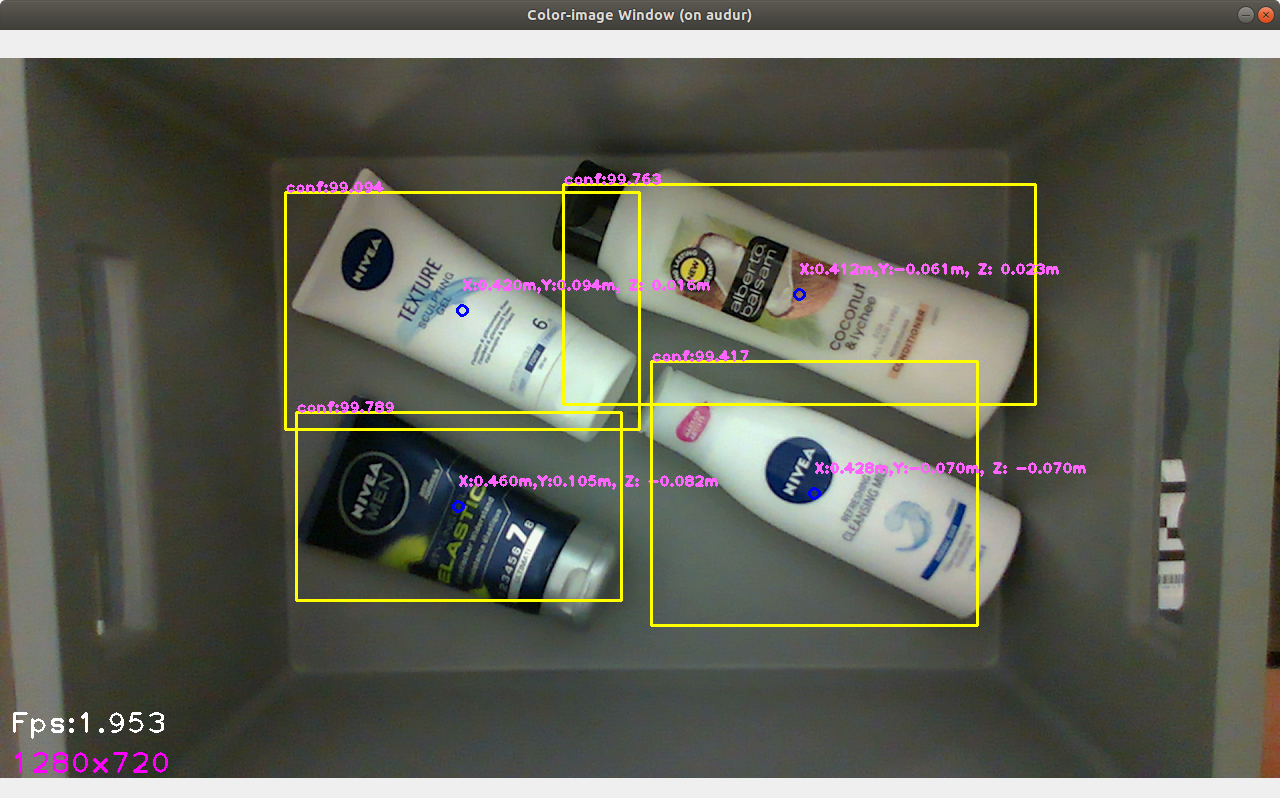
\includegraphics[width=0.33\textwidth]{graphics/results/aftertraining1.png}}
    \hfill
    \subfloat[Using trained YOLOv4]{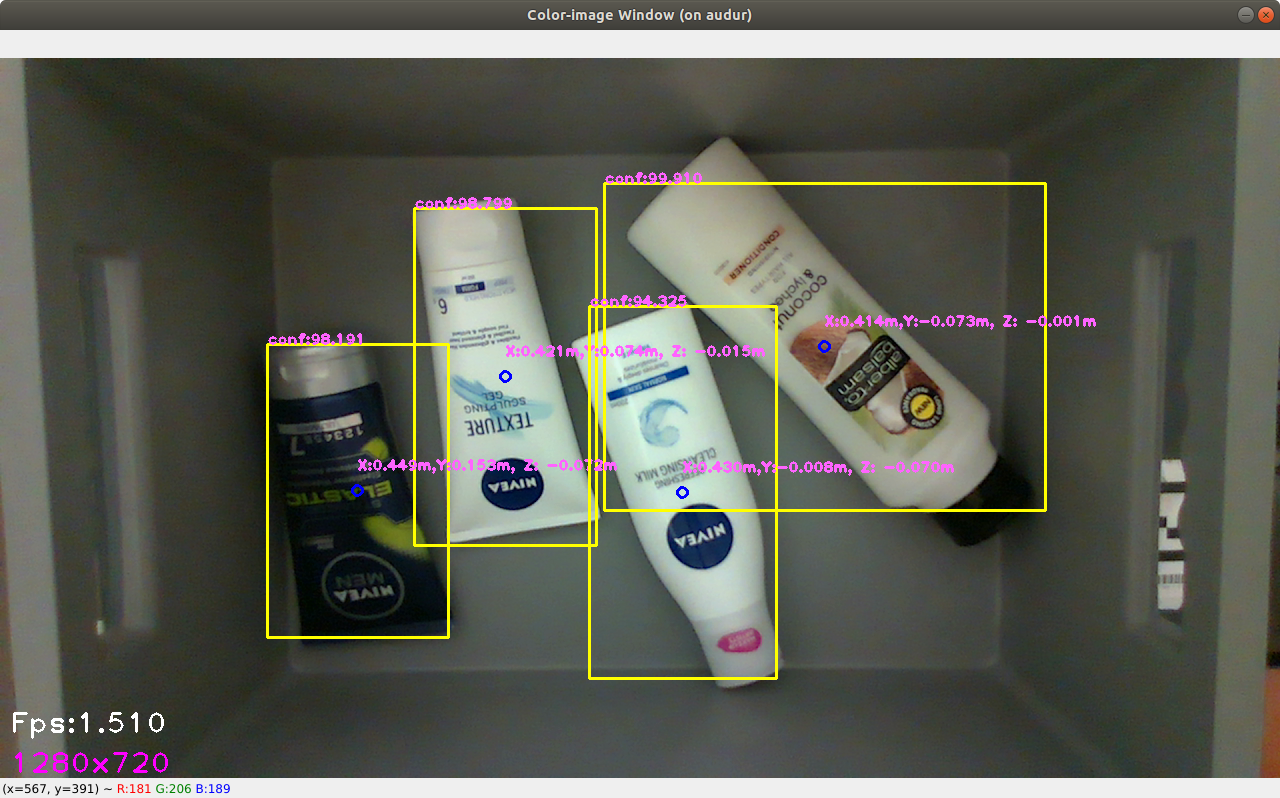
\includegraphics[width=0.33\textwidth]{graphics/results/aftertraining2.png}}
    \caption{Using YOLOv4 and the trained YOLOv4 model, trained on images from the robot}
    \label{figure: beforeaftertraining}
\end{figure}

% GPU: GeForce RTX 2080 Ti

% Net fra 25.04.21
% yolo-obj_new_1000.weights average for conf_thresh = 0.25, TP = 91, FP = 31, FN = 0, average IoU = 51.78 %
% yolo-obj_new_2000.weights average for conf_thresh = 0.25, TP = 91, FP = 0, FN = 0, average IoU = 84.03 %
% yolo-obj_new_3000.weights average for conf_thresh = 0.25, TP = 91, FP = 0, FN = 0, average IoU = 90.02 % 
% yolo-obj_new_4000.weights average for conf_thresh = 0.25, TP = 91, FP = 0, FN = 0, average IoU = 88.67 % 
% yolo-obj_new_5000.weights average for conf_thresh = 0.25, TP = 91, FP = 0, FN = 0, average IoU = 91.63 %
% yolo-obj_new_6000.weights average for conf_thresh = 0.25, TP = 91, FP = 0, FN = 0, average IoU = 91.84 %
% yolo-obj_new_7000.weights average for conf_thresh = 0.25, TP = 91, FP = 0, FN = 0, average IoU = 92.06 %
% yolo-obj_new_8000.weights average for conf_thresh = 0.25, TP = 91, FP = 0, FN = 0, average IoU = 92.88 %
% yolo-obj_new_9000.weights average for conf_thresh = 0.25, TP = 91, FP = 0, FN = 0, average IoU = 92.86 %
% yolo-obj_new_10000.weights average for conf_thresh = 0.25, TP = 91, FP = 0, FN = 0, average IoU = 91.63 % 
% yolo-obj_new_11000.weights average for conf_thresh = 0.25, TP = 91, FP = 0, FN = 0, average IoU = 82.79 %
% yolo-obj_new_12000.weights average for conf_thresh = 0.25, TP = 91, FP = 0, FN = 0, average IoU = 94.10 % BESTA NETIÐ
% yolo-obj_new_13000.weights average for conf_thresh = 0.25, TP = 91, FP = 0, FN = 0, average IoU = 94.01 %
% yolo-obj_new_14000.weights average for conf_thresh = 0.25, TP = 91, FP = 0, FN = 0, average IoU = 88.15 %
%yolo-obj_new_15000.weights average for conf_thresh = 0.25, TP = 91, FP = 0, FN = 0, average IoU = 92.48 % 

% yolo-obj_new_last.weights average for conf_thresh = 0.25, TP = 91, FP = 0, FN = 0, average IoU = 93.19 %

